% !TEX root = ../main.tex
\section{Spin-Boson Model as a Closed Reduced Generator}
\label{sec:qubit_closed_generator}\label{subsec:qubit_exact_geometry}

We now exhibit a case where all three compositional layers close exactly in the
spin-boson model~\cite{leggettDynamicsDissipativeTwostate1987,weissQuantumDissipativeSystems2012}.
This is the minimal genuinely noncommuting testbed: the adjoint orbit
terminates into a two-family alternation, the bilinear influence remains in the
Pauli algebra, and the full BCH tower resums to a closed generator. To our
knowledge, this yields the first closed-form Hamiltonian of mean force for a
genuinely noncommuting open quantum system. Earlier exact benchmarks are either
commuting, quadratic/Gaussian, or asymptotic; here the reduced generator stays
inside a finite operator algebra with no approximation at any stage.

Let us first set conventions. During derivation we work in the qubit energy
basis, $\hat{\mathbf n}_s=\hat{\mathbf z}$, and then rewrite the final answer
covariantly in the coupling plane spanned by $\hat{\mathbf n}_s$ and
$\hat{\mathbf f}$. We take
\begin{equation}
    H_Q = \frac{\omega_q}{2}\,\hat{\mathbf n}_s\!\cdot\!\boldsymbol{\sigma},
    \qquad
    f = \hat{\mathbf f}\!\cdot\!\boldsymbol{\sigma},
\end{equation}
with $\hat{\mathbf f}=(s\cos\phi,s\sin\phi,c)$, $c\equiv\cos\theta$,
$s\equiv\sin\theta$. The overall coupling amplitude $g$ is suppressed in
intermediate expressions and reintroduced when discussing scaling.

\subsection{Bath kernels and the symmetrized influence state}
\label{subsec:qubit_influence_state}

The interaction-picture coupling operator is
\begin{equation}
    \tilde f(\tau)=e^{\tau H_Q}fe^{-\tau H_Q}
    = c\sigma_z + f_-e^{\omega_q\tau}\sigma_+ + f_+e^{-\omega_q\tau}\sigma_-,
\end{equation}
with $f_\pm=s e^{\pm i\phi}$. The Pauli algebra then implies that all bath
dependence enters through two real response channels,
\begin{equation}
    \begin{aligned}
    \Sigma_z &\equiv \frac{1}{2}\!\left[R(\omega_q)-R(-\omega_q)\right], \\
    \Sigma_\perp &\equiv \frac{4}{\omega_q}\!\left[
        \cosh\!\left(\frac{\beta\omega_q}{2}\right)\mathcal K(0)
        -e^{-\beta\omega_q/2}\mathcal K(\omega_q)\right].
    \end{aligned}
    \label{eq:bath_kernels_direct}
\end{equation}
The reduced operator can be written in the symmetrized form
$\bar\rho_Q=\Pi^{1/2}e^S\Pi^{1/2}$, with $\Pi=e^{-\beta H_Q}$ and
\begin{equation}
    S=\Delta_0\mathbb I
    +s^2\Sigma_z\,\sigma_z
    -sc\,\Sigma_\perp(\cos\phi\,\sigma_x+\sin\phi\,\sigma_y).
    \label{eq:S_symmetrised_v3}
\end{equation}
Subtracting the scalar piece, $M\equiv S-\Delta_0\mathbb I$, gives an influence
Bloch vector
\begin{equation}
    \mathbf m_S=
    s\Sigma_\perp\hat{\mathbf f}_\perp + s^2(\Sigma_z-\Sigma_\perp)\hat{\mathbf n}_s,
    \label{eq:mS_decomposition}
\end{equation}
where $\hat{\mathbf f}_\perp=(-c\cos\phi,-c\sin\phi,s)$ lies in the coupling
plane and is orthogonal to $\hat{\mathbf f}$.

The corresponding influence magnitude is
\begin{equation}
    \chi=\|\mathbf m_S\|
    = |s|\sqrt{c^2\Sigma_\perp^2+s^2\Sigma_z^2},
    \label{eq:chi_factored}
\end{equation}
and the normalized influence state is
\begin{equation}
    \rho_S=\frac{e^S}{\Tr(e^S)}
    = \frac{1}{2}\!\left[\mathbb I+\tanh\chi\,\hat{\mathbf m}_S\!\cdot\!\boldsymbol{\sigma}\right],
    \qquad
    \hat{\mathbf m}_S=\mathbf m_S/\chi.
    \label{eq:expS_closed}
\end{equation}
Its tilt inside the coupling plane is fixed by the ratio of response channels,
\begin{equation}
    \tan\varphi_S=-\,\frac{c}{s}\,\frac{\Sigma_\perp}{\Sigma_z}.
    \label{eq:phiS_def}
\end{equation}
At this stage the constructive content is already visible: the entire bath has
compressed to two scalar channels and one influence magnitude. The first two
compositional layers have therefore already closed: the adjoint orbit has
collapsed into finitely many Pauli directions, and the bilinear influence has
compressed into a finite set of response coefficients.

\subsection{Closed reduced state and generator}
\label{subsec:qubit_closed_generator}

Recombining the influence state with the bare Gibbs factor yields the reduced
state
\begin{equation}
    \rho_Q = \frac{1}{2}\big[\mathbb I + r_Q \hat{\mathbf m}_Q \cdot \boldsymbol{\sigma}\big],
    \label{eq:rho_matrix_general}
\end{equation}
with Bloch components
\begin{equation}
    m_z = r_Q\cos\varphi_Q,
    \qquad
    m_\perp = r_Q\sin\varphi_Q.
    \label{eq:tilt_angle_def}
\end{equation}
The longitudinal scale is controlled by
\begin{align}
    \Theta &\equiv
    \operatorname{arctanh}\!\big(\gamma(\chi)\,s^2\Sigma_z\big)
    -\frac{\beta\omega_q}{2},
    \label{eq:theta_param} \\
    \gamma(\chi) &\equiv \tanh\chi/\chi,
\end{align}
which gives the exact solution
\begin{align}
    m_z &= \tanh\Theta,
    \label{eq:m_z_solution} \\
    m_\perp &= \tan\varphi_S\!\left(
        m_z\cosh\frac{\beta\omega_q}{2}
        +\sinh\frac{\beta\omega_q}{2}\right).
    \label{eq:bloch_locking_linear}
\end{align}
The final tilt and radius follow as
\begin{equation}
    \tan\varphi_Q = \tan\varphi_S\,
    \frac{m_z + r_0}{\sqrt{1-r_0^2}\;m_z},
    \qquad
    r_0=\tanh\!\left(\frac{\beta\omega_q}{2}\right),
    \label{eq:phiQ_def}
\end{equation}
and
\begin{equation}
    1-r_Q^2
    = \frac{(1-r_0^2)(1-r_S^2)}{(1+r_0 r_S\cos\varphi_S)^2},
    \qquad
    r_S=\tanh\chi.
    \label{eq:rQ_geometric_composition}
\end{equation}
Figure~\ref{fig:bloch_overview} summarizes this Bloch-plane geometry while
Eqs.~\eqref{eq:m_z_solution}--\eqref{eq:rQ_geometric_composition} are being
parsed: the bare Gibbs state, the symmetrized influence state, and the final
reduced state all remain in a single plane fixed by the system and coupling
axes.

\begin{figure}[!t]
    \centering
    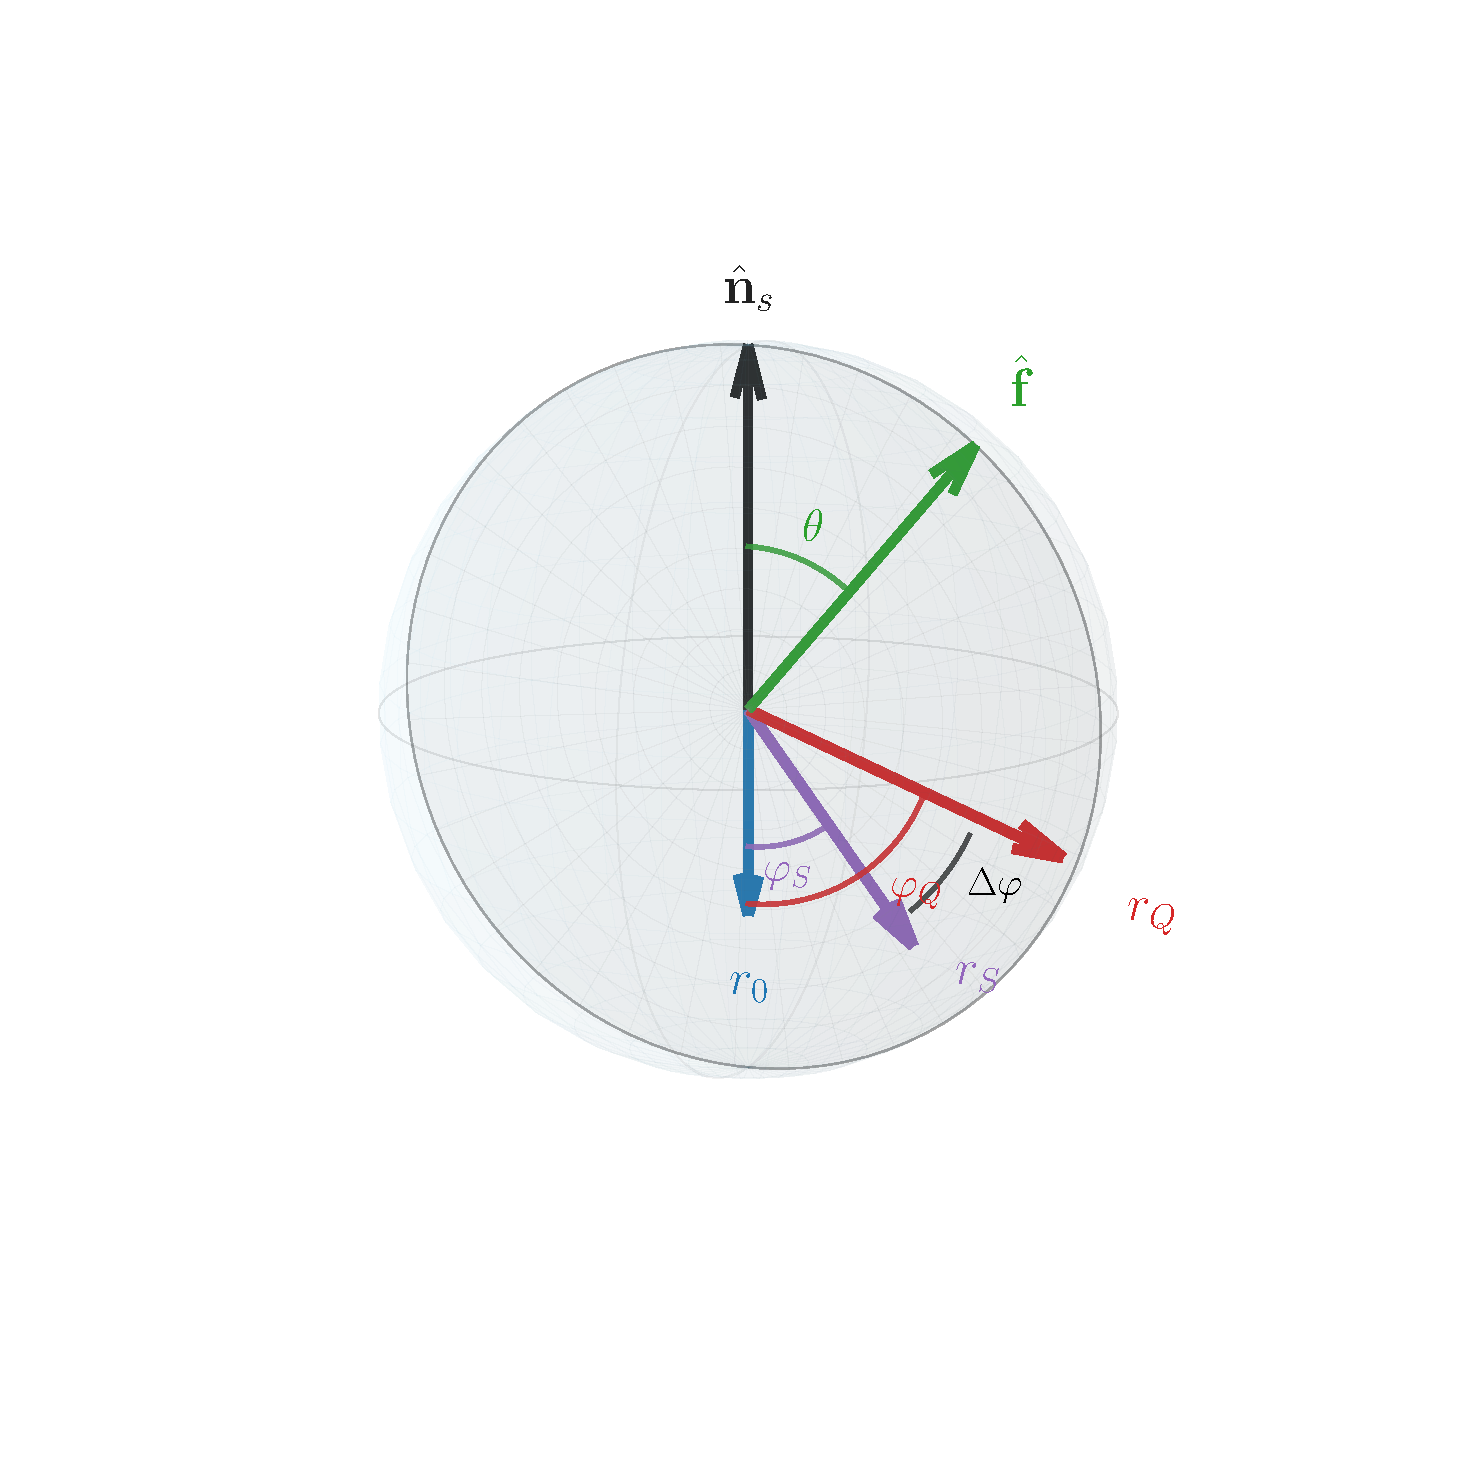
\includegraphics[width=0.84\columnwidth]{../figures/hmf_bloch_3d_overview.pdf}
    \caption{Bloch-plane geometry for the exact qubit construction. The bare
    thermal state has radius $r_0$ (blue), the symmetrized influence state has
    radius $r_S$ and tilt $\varphi_S$ (purple), and the final reduced state has
    radius $r_Q$ and tilt $\varphi_Q$ (red). The exact generator never leaves
    the system--coupling plane.}
    \label{fig:bloch_overview}
\end{figure}

For any full-rank qubit state, the operator logarithm is elementary. Writing
$\hat{\mathbf m}_Q=(m_\perp\cos\phi,m_\perp\sin\phi,m_z)/r_Q$, the exact qubit
Hamiltonian of mean force is therefore
\begin{equation}
    H_{\mathrm{MF}}(\beta)
    = h_0(\beta)\,\mathbb I
    - \frac{1}{\beta}\operatorname{arctanh}(r_Q)\,
      \hat{\mathbf m}_Q\!\cdot\!\boldsymbol{\sigma},
    \label{eq:HMF_qubit_closed_hmf_ai}
\end{equation}
where the scalar $h_0(\beta)$ fixes normalization and carries the additive
identity freedom of the HMF. Equation~\eqref{eq:HMF_qubit_closed_hmf_ai} makes
the closure statement concrete: the exact reduced generator remains inside the
same Bloch-plane operator family throughout, while the bath enters only through
the two response channels $(\Sigma_z,\Sigma_\perp)$ and the influence scale
$\chi$. This is the fully closed instance of the compositional proposition:
the adjoint orbit terminates, the bilinear aggregation closes in the Pauli
algebra, and the nonlinear BCH sector resums because the traceless influence
obeys $M^2=\chi^2\mathbb I$.
